\documentclass[12;pt,t]{beamer} % beamer - typ/šablona prezentace

\usepackage[english]{babel} % nastavuje české popisky např. u obsahu, referencí, tabulek, obázků 
\usepackage[utf8]{inputenc} % použito UTF8 kvůli češtině (zvládá prakticky všechny jazyky na světě)
\usepackage[T1]{fontenc}

\usepackage{lmodern}
%\usepackage{datetime}
\usepackage{amssymb} % podpůrná knihovna pro matematické symboly
\usepackage{enumerate} % umožňuje širší možnosti nastavení enumerate

\usepackage{graphicx} % vkládání obrázků
\usepackage{hologo} % logo BibTeX

\usepackage{multicol} % pro praci s více sloupci

\usepackage{xcolor}
\usepackage{listings}

\lstset{basicstyle=\footnotesize\ttfamily,
  showstringspaces=false,
  commentstyle=\color{red},
  keywordstyle=\color{blue},
  escapeinside={(*@}{@*)},
  breaklines=true,
  extendedchars=true,
  inputencoding=utf8
}

\lstdefinelanguage{bettertex}{%
  language     = tex,
  morekeywords = {begin,hline},
}

% pro pěkné zobrazení zdroje obrázků
\definecolor{sourcesclr}{rgb}{.38,.38,.38}
\newcommand{\srctext}[1]{{\fontsize{7}{9}\selectfont\textcolor{sourcesclr}{#1}}}

% Themes: http://www.hartwork.org/beamer-theme-matrix/
\mode<presentation>{\usetheme{Madrid}}
\usecolortheme{beaver}
\beamertemplatenavigationsymbolsempty 
\setbeamertemplate{title page}[default][colsep=0bp,rounded=true]
\setbeamertemplate{itemize items}{-} %$\circ$
\setbeamercolor*{item}{fg=black}
\setbeamertemplate{enumerate item}[default]


\author{Jaroslav Páral}
\institute[paral.jarek@gmail.com]{FI MUNI: PB174\\[0.5cm]}
\title{Energy harvesting - solar energy}


\begin{document}

\frame{\titlepage}

\begin{frame}
    \frametitle{Introduction}
    	\begin{figure}[H]
            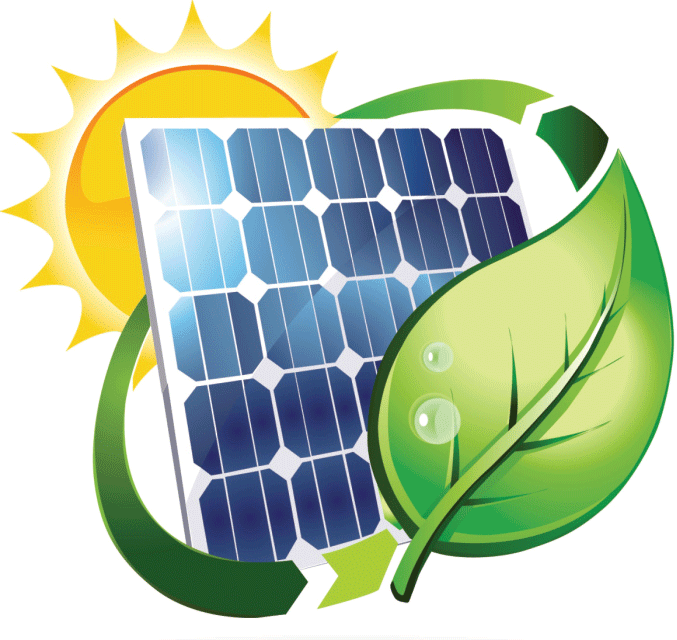
\includegraphics[width=190px]{img/Energy-harvesting.png}
            %\caption{Harvesting of the solar energy}
    	\end{figure}
    	    \srctext{Image source: \url{http://electronicsmaker.com/energy-harvesting-for-iot-wireless-applications}}
\end{frame}

\begin{frame}
    \frametitle{Problem with solar energy}
		\begin{itemize}
			\item Sun (energy provide from the sunrise to sunset)
			\item Weather (clouds, snow, temperature)
			\item Season (summer/winter)
            \item Efficiency of photo-voltaic panels (10 - 15 \%)
            \item Efficiency in time  
     		\item Required energy by device
            \item Energy use (=> accumulate)
            \item Efficient accumulation
       \end{itemize}
\end{frame}

\begin{frame}
    \frametitle{Harvesting of solar energy - many elements}    	
        \begin{figure}[H]
            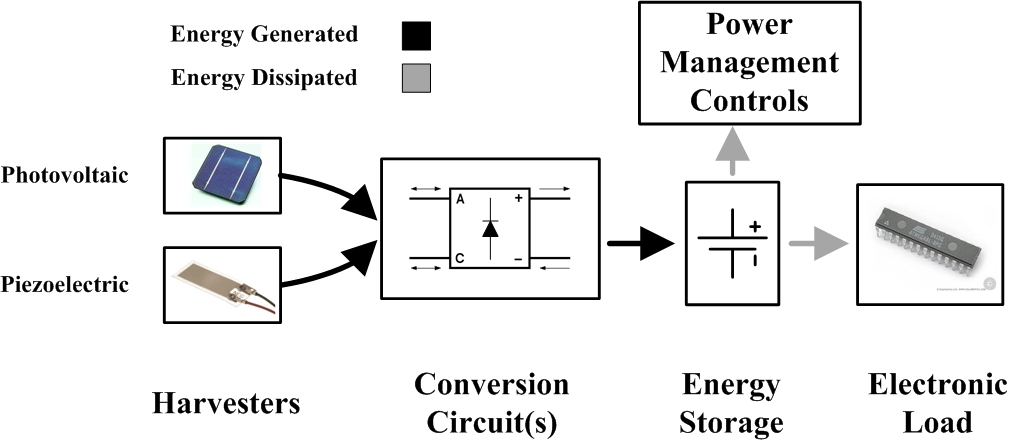
\includegraphics[width=320px]{img/energy_harvesting_block_diagram.png}
            %\caption{Harvesting of the solar energy}
       	\end{figure}
    \srctext{Image source: \url{http://www.mae.cornell.edu/research/groups/lims/research/lab_on_a_bird.cfms}}
\end{frame}

\begin{frame}
    \frametitle{Solar energy => photovoltaic panel (1)}
    Solar energy (maximum usable energy from the sun): $1000 W/m^2$\\
    Efficiency of photo-voltaic panels: 10 - 15 \%\\ 
    
   \vspace{5mm}
    1 $dm^2$ solar panel (10 \%) => 10 W (theoretical max output)\\
    
    Tests with real panel:
    \begin{center}
   		\begin{enumerate} %[<+->]
   			\item Maximum ($1000 W/m^2$) = 100 \%
  			\item Best weather condition =  33 \%
   			\item April - September = 21 \%
   			\item October - March = 10 \%
  			\item December - January = 4 \%
            \item Year average = 14 \%
   		\end{enumerate}
    \end{center}
    \srctext{Data source: \url{https://is.muni.cz/th/359790/fi_b/}}
\end{frame}

\begin{frame}
    \frametitle{Solar energy => photovoltaic panel (2)}
        \begin{figure}[h]
           	\begin{minipage}[b]{.42\textwidth}
           		\centering
           		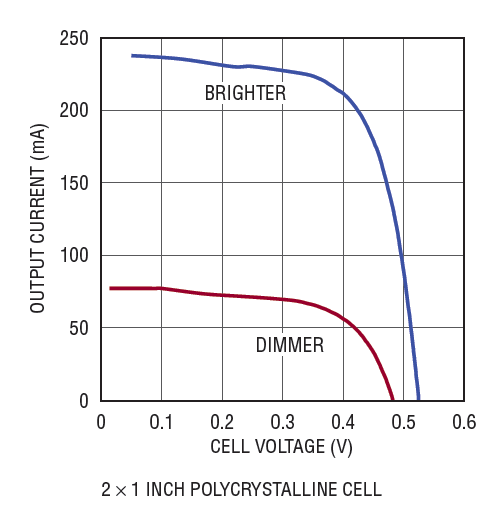
\includegraphics[width=\textwidth]{img/photovoltaic-panel-AV-char.png}
                \caption{V-A characteristic}
           	\end{minipage}
           	\hfill
           	\begin{minipage}[b]{.42\textwidth}
           		\centering
           		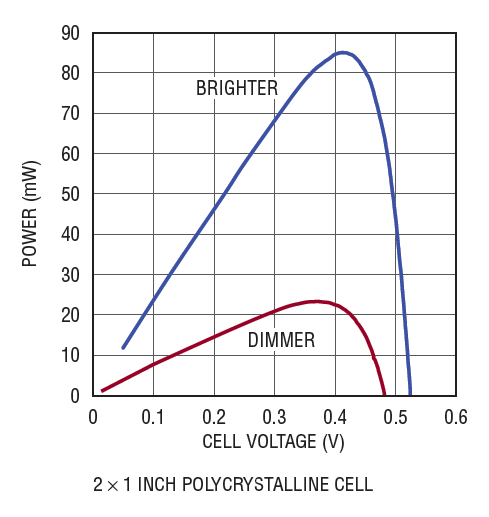
\includegraphics[width=\textwidth]{img/photovoltaic-panel-WV-char.png}
                \caption{V-W characteristic}
           	\end{minipage}
        \end{figure}
    \srctext{Image source: \url{https://vyvoj.hw.cz//firemni-clanky/sos-electronic/ltc3105-solarni-zne-v-praxi-1-cast.html}}
\end{frame}

\begin{frame}
    \frametitle{Solar energy => photovoltaic panel (3)}
        \begin{figure}[h]
      		\centering
       		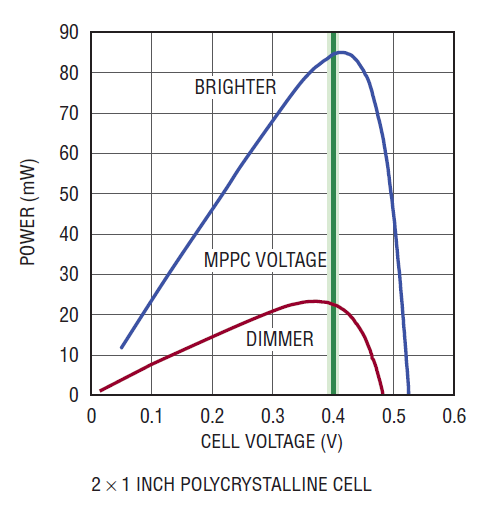
\includegraphics[width=150px]{img/photovoltaic-panel-WV-char-MPP.png}
            \caption{V-W characteristic - MPP (Maximum Power Point)}
        \end{figure}

    \srctext{Image source: \url{https://vyvoj.hw.cz//firemni-clanky/sos-electronic/ltc3105-solarni-zne-v-praxi-2-cast.html}}
\end{frame}

\begin{frame}
    \frametitle{Harvesting of solar energy - many elements}    	
        \begin{figure}[H]
            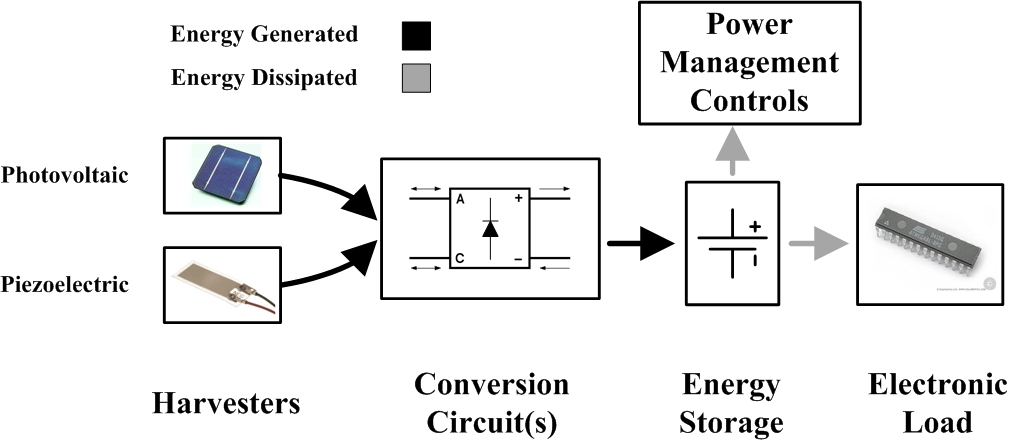
\includegraphics[width=320px]{img/energy_harvesting_block_diagram.png}
            %\caption{Harvesting of the solar energy}
       	\end{figure}
    \srctext{Image source: \url{http://www.mae.cornell.edu/research/groups/lims/research/lab_on_a_bird.cfms}}
\end{frame}

\begin{frame}
    \frametitle{Electronic load}
    \begin{center}
		\begin{enumerate}
			\item Hardware 
                \begin{itemize}
                    \item MCU
                    \item sensors
                    \item communication module
                \end{itemize}
			\item Usage
                \begin{itemize}
                    \item period of measuring
                    \item period of sending date
                \end{itemize}
			\item Other elements
                \begin{itemize}
                    \item interference
                    \item temperature
                \end{itemize}
        \end{enumerate}
    \end{center}
\end{frame}

\begin{frame}
    \frametitle{Electronic load - communication}    	
        \begin{figure}[H]
            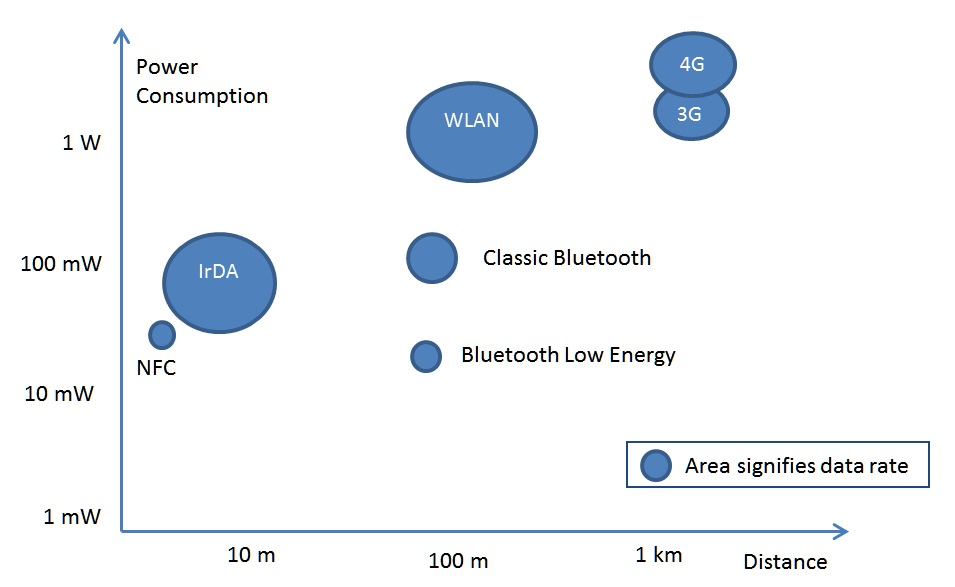
\includegraphics[width=300px]{img/consuption-of-comunication-tech.jpg}
            %\caption{Harvesting of the solar energy}
       	\end{figure}
    \srctext{Image source: \url{https://goo.gl/exzYSa}}
\end{frame}


\begin{frame}
    \frametitle{Energy storage}
    \begin{center}
		\begin{enumerate}
			\item capacity
            \item max. input current 
            \item max. output current 
            \item self-discharge
		\end{enumerate}
    \end{center}
    
    \begin{figure}[H]
        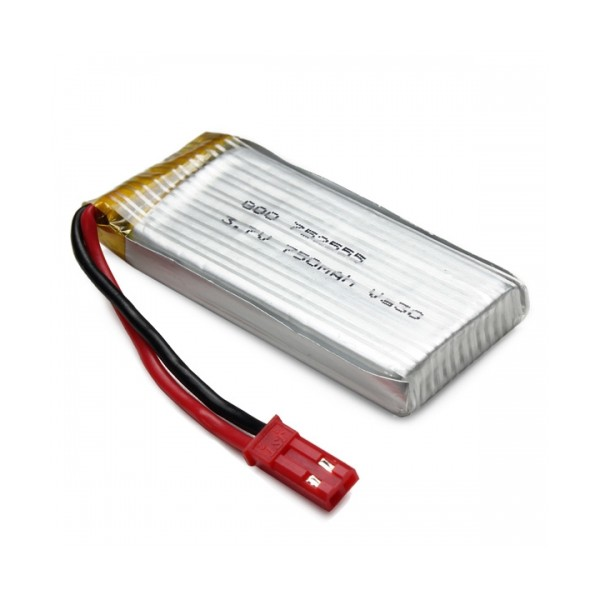
\includegraphics[width=120px]{img/li-pol-akumulator-pro-dron-sky-boot-700mah-37v.jpg}
        %\caption{Harvesting of the solar energy}
   	\end{figure}
    \srctext{Image source: \url{http://rcsale.cz/akumulatory-a-baterie/129-li-pol-akumulator-pro-syma-x5c-a-x5w-37v-500mah.html}}
\end{frame}


\begin{frame}
    \frametitle{Conversion circuit}
    Two types:
    	\begin{enumerate}[A)]
			\item linear
            \item step-up
    	\end{enumerate}
   
   \vspace{5mm}
   Parameters:
 	\begin{itemize}
		\item own consumption
        \item efficient
        \item input voltage
        \item MPP (Maximum Power Point)?
   	\end{itemize}

\end{frame}

\begin{frame}
    \frametitle{Conversion circuit - linear}
    Example: MCP73831
   
   \vspace{5mm}
   Parameters:
 	\begin{itemize}
		\item prize: 0.5 Euro
        \item input: 4.25 – 6.5 V
        \item max output: 800 mA
        \item without MPP
   	\end{itemize}
    \srctext{Source: \url{http://uk.farnell.com/microchip/mcp73831t-2aci-ot/li-ion-li-poly-charge-controller/dp/1332158}}
\end{frame}

\begin{frame}
    \frametitle{Conversion circuit - MCP73831 - Typical Application}    	
        \begin{figure}[H]
            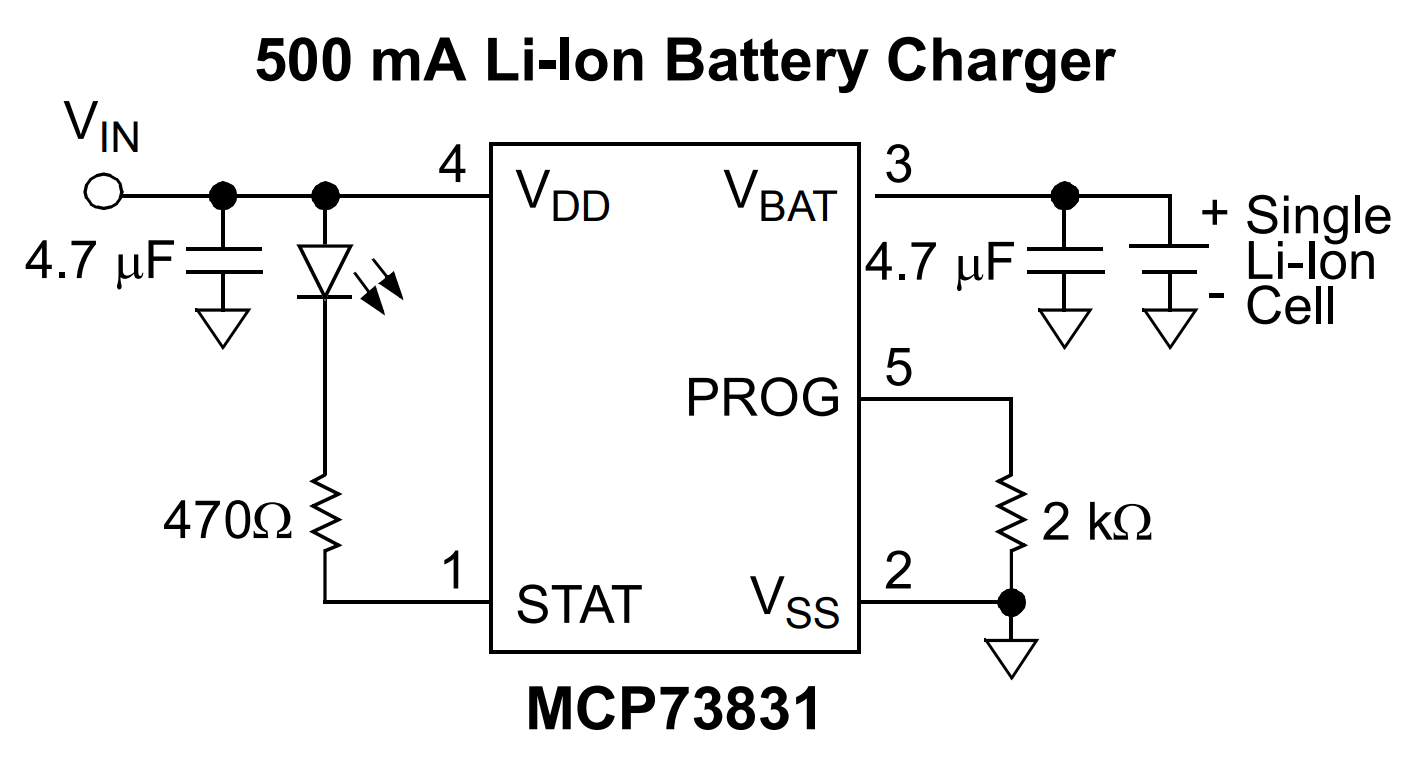
\includegraphics[width=290px]{img/mcp73831-base-circuit.png}
            %\caption{Harvesting of the solar energy}
       	\end{figure}
    \srctext{Image source:  \url{https://vyvoj.hw.cz//firemni-clanky/sos-electronic/ltc3105-solarni-zne-v-praxi-2-cast.html}}
\end{frame}


\begin{frame}
    \frametitle{Conversion circuit - step-up}
    Example: LTC3105
   
   \vspace{5mm}
   Parameters:
 	\begin{itemize}
		\item prize: 5 Euro
        \item input: 0.25 – 5 V
        \item output: 1.2 – 5.25 V
        \item max output: 400 mA
        \item with MPP
   	\end{itemize}
    \srctext{Source: \url{https://www.soselectronic.cz/products/linear-technology/ltc3105ems-pbf-129761}}
\end{frame}

\begin{frame}
    \frametitle{Conversion circuit - LTC3105 - Typical Application}    	
        \begin{figure}[H]
            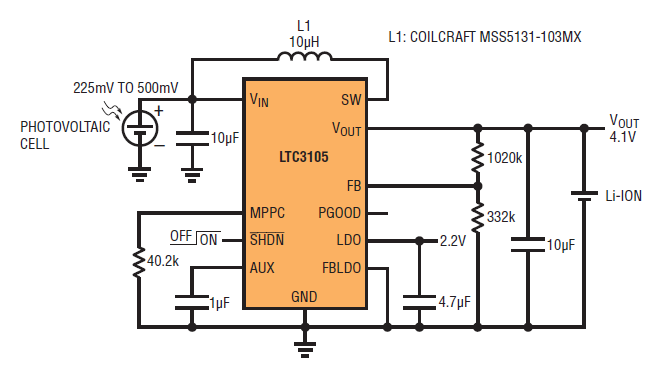
\includegraphics[width=290px]{img/ltc3105-base-circuit.png}
            %\caption{Harvesting of the solar energy}
       	\end{figure}
    \srctext{Image source:  \url{https://vyvoj.hw.cz//firemni-clanky/sos-electronic/ltc3105-solarni-zne-v-praxi-2-cast.html}}
\end{frame}


\begin{frame}
    \frametitle{Conversion circuit - LTC3105 - Electronic load}    	
        \begin{figure}[H]
            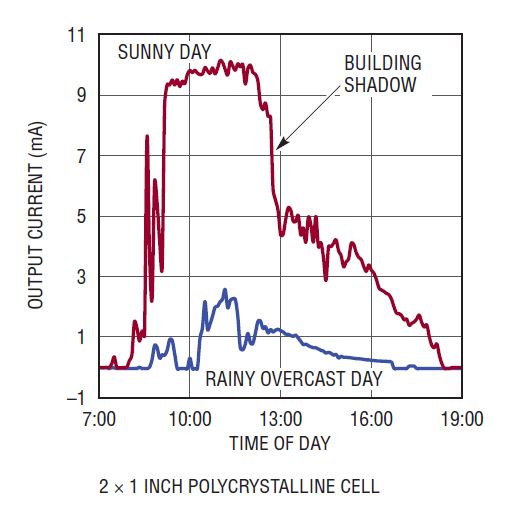
\includegraphics[width=180px]{img/ltc3105-base-circuit-graph.png}
            %\caption{Harvesting of the solar energy}
       	\end{figure}
    \srctext{Image source:  \url{https://vyvoj.hw.cz//firemni-clanky/sos-electronic/ltc3105-solarni-zne-v-praxi-2-cast.html}}
\end{frame}

\begin{frame}[fragile]
	\vfill
    \begin{center}
        {\huge Thank you for your attention }
	\end{center}
	\vfill
\end{frame}


\end{document}

